\documentclass[a4paper]{article}
\usepackage[utf8]{inputenc}
\usepackage[a4paper, left=15mm, top=20mm, right=15mm]{geometry}

\usepackage{multirow}
\usepackage{pdflscape}
\usepackage{subfiles}

% allows for temporary adjustment of side margins
\usepackage{chngpage}

\title{Libretto vecchi lupi VdB 2016}
\author{Staff}
\date{31 Luglio / 7 Agosto 2016}

\usepackage{natbib}
\usepackage{graphicx}

\begin{document}

\begin{titlepage}
\begin{figure}[p]
    \vspace*{-2cm}
    \makebox[\linewidth]{
        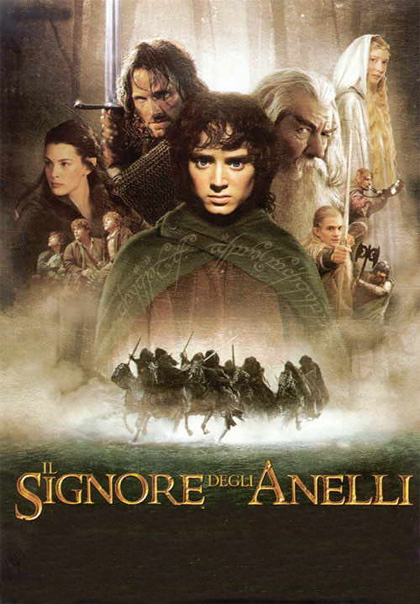
\includegraphics[width=1.2\linewidth]{locandina.jpg}
    }\end{figure}
\end{titlepage}

\begin{landscape}
\begin{adjustwidth}{-2.5cm}{-1cm}% adjust the L and R 
 \begin{tabular}{|r|c|c|c|c|c|c|c|c|}
 \hline
 \multicolumn{9}{|c|}{Vacanze di Branco 2016}\\
 \hline
        &Dom 31 Luglio&Lun 1 Agosto&Mar 2 Agosto&Mer 3 Agosto&Giò 4 Agosto&Ven 5 Agosto&Sab 6 Agosto&Dom 7 Agosto\\ \hline
        07:30& &Sveglia&Sveglia&Sveglia&Sveglia&Sveglia&Sveglia&Sveglia\\ \hline
        
        % -- Prima riga con colazione, ginnastica, lavaggi e ispezione
        \multirow{2}{*}{08:00 - 10:00}&Ritrovo&Ginnazio+Colazio&Ginnazio+Colazio&Ginnazio+Colazio&Ginnazio+Colazio&Ginnazio+Colazio&Ginnazio+Colazio&Ginnazio+Colazio\\
        &Verifica+propositi&Lavazio+Ispezio&Lavazio+Ispezio&Lavazio+Ispezio&Lavazio+Ispezio&Lavazio+Ispezio&Lavazio+Ispezio&Zainazio\\ \hline
        
        %% -- Seconda riga con attività della mattina
        \multirow{2}{*}{10:00 - 12:30}&Messa&Rifugi mistiglie&Caccia&Bottega&Bottega&Giochi d'H2O + Doccia&Bottega&Verifica\\
        & &Urlo+Stemma& & & & & &\\ \hline
        
        % -- Terza riga con pranzo
        \multirow{2}{*}{12:30 - 15:00}&Pappa+carico&Pranzo+Servizi&Pranzo&Pranzo+Servizi&Pranzo+Servizi&Pranzo+Servizi&Pranzo+Servizi&Pranzo\\&Via!&TL&TL&TL&TL&TL&TL&\#SalutiEPianti\\ \hline
    
        % -- Quarta riga - Primo pomeriggio
        \multirow{2}{*}{15:00 - 16:30}&Arrivo&Compagnia&Racconto&Cluedo&Gioco Battaglia&Bottega&Caccia al tesoro&Pranzo+Pulizie\\& &dell'anello&2& & & & &\\ \hline
        
        % &Arrivo&Compagnia&Racconto&Cluedo&Gioco Battaglia&Bottega&Caccia al tesoro&Pranzo+Pulizie
    
        % -- Quinta riga - Catechesi
        \multirow{2}{*}{16:30 - 17:30}&Salita al posto&Merenda&Gioco&Merenda&Merenda&Merenda&Merenda&\\& &Catechesi&Giungla 2&Catechesi&Catechesi&Catechesi&Catechesi&\\ \hline
        \multirow{2}{*}{17:30 - 19:30}&Regole+servizi&(O)GM&Doccia&(O)GM&(O)GM&(O)GM&(O)GM&\\&+zaini& & & & & & &\\ \hline
        
        % -- Sesta riga - Cenae
        19:30 - 21:00&Cena&Cena&Cena&Cena&Cena&Cena&Cena&\\ \hline      
        % -- Settima riga - Fuochi
        \multirow{2}{*}{21:00 - 22:30}&Tema+Mistiglie&Fuoco 1&C.d'atmosfera&GiocoNotturno&Fuoco 2&Veglia alle stelle&Fiesta&\\&Posta+canzone& & & & & & & \\\hline        

        % -- Ottava riga - Nanna!
        22:30&Nanna&Nanna&Nanna&Nanna&Nanna&Nanna&Nanna&\\ \hline
        \end{tabular}  
        \end{adjustwidth}
\end{landscape}

\newpage
    \subfile{subsections/domenica_31.tex}
\newpage
    \subfile{subsections/lunedi_1.tex}
\newpage
    \subfile{subsections/martedi_2.tex}
\newpage
    \subfile{subsections/mercoledi_3.tex}
\newpage
    \subfile{subsections/giovedi_4.tex}
\newpage
    \subfile{subsections/venerdi_5.tex}
\newpage
    \subfile{subsections/sabato_6.tex}
\newpage
    \subfile{subsections/domenica_7.tex}
\newpage
    \subfile{subsections/botteghe.tex}
    \subfile{subsections/personaggi.tex}

\end{document}
